\documentclass[10pt]{beamer}
\usetheme{Pecnum}
\usepackage{amsmath,amssymb}
\usepackage{colortbl}
%\usepackage{ucs}
\usepackage[utf8]{inputenc}
\usepackage{textcomp}
\usepackage{amsfonts,amssymb,amsmath,amsthm,amsbsy}
\usepackage{placeins}
\usepackage{color}
\usepackage{tikz}
\usepackage{bbm}

\setbeamercovered{dynamic}
\setbeamercolor{postit}{bg=pecnumbleusombre!30}
\title{Stratégies séquentielles}
\author{Victor Picheny}
\date{\'Ecole Centrale de Lyon, 22 mai 2015}
\institute{\includegraphics[scale=.15]{logo.png}}

\begin{document}
\begin{frame}
    	\maketitle
\end{frame}

%-----------------------------------------------------------------
%%%%%%%%%%%%%%%%%%%%%%%%%%%%%%%%%%%%%%%%%%%%%%%%%%%%%%%%%%%%%%%%%%
%-----------------------------------------------------------------
\section{Introduction}
%-----------------------------------------------------------------
\begin{frame}{Cadre de l'exposé}
 \includegraphics[width=\textwidth]{fig/schemaSeb.png}
\end{frame}

%-----------------------------------------------------------------
\begin{frame}{Pourquoi une stratégie séquentielle ?}
\begin{block}{``Budget'' ($=N$) nécessaire difficile à estimer}
\begin{itemize}
  \item Premier plan raisonnable
  \item Enrichissement jusqu'à satisfaction
\end{itemize}
\end{block}

\begin{alertblock}{Suite d'une première étude}
\begin{itemize}
\item Premier plan $\Rightarrow$ métamodèle grossier $\Rightarrow$ analyse de sensibilité $\Rightarrow$ réduction de dimension
\item Ajout d'expériences pour obtenir un métamodèle final précis
\end{itemize}
\end{alertblock}

\begin{exampleblock}{Planification ciblée $\Leftrightarrow$ utilisation du métamodèle}
\begin{itemize}
\item Propagation d'incertitudes
\item Analyse de sensibilité
\item Optimisation / calibration
\end{itemize}
\end{exampleblock}
\end{frame}
%-----------------------------------------------------------------
\begin{frame}{Approches géométriques vs. métamodèles}

\textbf{Comment ajouter des expériences à un plan existant ?}

\vspace{5mm}

\begin{block}{Approches ``purement'' géométriques}
  \begin{itemize}
  \item Plan factoriels fractionnaires $\Rightarrow$ ajout d'une fraction
  \item Suite à faible discrépance $\Rightarrow$ éléments suivants
  \item Remplissage d'espace (critères \textit{maximin}, \textit{minimax})
 \end{itemize}
$\Rightarrow$ c.f. cours de W. Tinsson, H. Monod et L. Pronzato
\end{block}

\begin{alertblock}{Ici : plans séquentiels \emph{\textit{orientés modèle}}}
 Le métamodèle sert de guide pour choisir les nouvelles observations.
\end{alertblock}
\end{frame}
%-----------------------------------------------------------------
\begin{frame}{Objectifs}
\begin{block}{Cas 1 : métamodèle globalement précis}
Utilisation générique $\Rightarrow$ le métamodèle doit remplacer fidèlement le modèle coûteux
\end{block}

\begin{exampleblock}{Cas 2 : métamodèle = outil d'extraction d'une information}
Intérêt guidé par la valeur des observations
\begin{itemize}
 \item optimisation : recherche de minimum / maximum
 \item analyse de risque : dépassement de seuil
\end{itemize}
Une bonne précision partout n'est pas nécessaire !
\end{exampleblock}
\end{frame}
%-----------------------------------------------------------------
%-----------------------------------------------------------------
\section[Prédiction]{Planification adaptative pour la prédiction}
%-----------------------------------------------------------------
\begin{frame}{Plan de l'exposé}
\tableofcontents
\end{frame}
%-----------------------------------------------------------------
\input{prediction.tex}
%-----------------------------------------------------------------
\section[Analyse de risque]{Planification adaptative pour l'analyse de risque}
%-----------------------------------------------------
\begin{frame}{Plan de l'exposé}
\tableofcontents
\end{frame}
%-----------------------------------------------------------------
\begin{frame}{Motivation}
\begin{block}{Apprentissage global ou ``ciblé''}
\begin{itemize}
 \item Le plan d'expérience a une influence très forte sur la précision locale
 \item Une bonne précision n'est pas nécessaire partout !
\end{itemize}
\end{block}

\begin{figure}
\centering
\includegraphics[width=\textwidth]{figT/two7pointskrigs.png} 
\end{figure}

\begin{alertblock}{Dans cette section}
 Un \textit{exemple} de plan séquentiel adapté à l'objectif
\end{alertblock}
\end{frame}

%%%%%%%%%%%%%%%%%%%%%%%%%%%%%%%%%%%%%%%%%%%%%%%%%%%%%%%%%%%%%%%%%%%%%%%%%%%%%%%%%%%%%%%%%%%%%%%%
\begin{frame}{Propagation d'incertitudes et analyse de risque (1/2)}
\begin{block}{Un problème classique : dépassement de seuil}
\begin{itemize}
 \item La sortie du simulateur doit rester sous une valeur critique (contraintes mécaniques, température, etc.)
 \item On connaît la loi des paramètres d'entrée
 \item On veut estimer : $\mathbb{P}\left[ y(X)\right] \geq seuil$
\end{itemize}
\end{block}

\vspace{10mm}
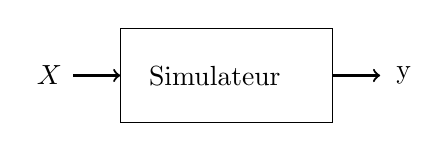
\begin{tikzpicture}[scale=0.3]
  \draw(0,1) node{$X$ };
   \draw[->,thick] (1,1)--(3,1);
  \draw(3,-1) rectangle (12,3);
  \draw(7,1) node{Simulateur};
 \draw[->,thick] (12,1)--(14,1);
 \draw(15,1) node{y};
 \end{tikzpicture}

\end{frame}
%%%%%%%%%%%%%%%%%%%%%%%%%%%%%%%%%%%%%%%%%%%%%%%%%%%%%%%%%%%%%%%%%%%%%%%%%%%%%%%%%%%%%%%%%%%%%%%%
\begin{frame}{Propagation d'incertitudes et analyse de risque (2/2)}
\begin{itemize}
 \item Approche par Monte-Carlo : on génère $X_1, \ldots, X_N$ $\Rightarrow$ $y(X_1), \ldots, y(X_N)$ et on compte 
 $$\frac{1}{N}\sum_{i=1}^N \mathbbmss{1}(y(X_i)) > T$$
\begin{figure}
\centering
\includegraphics[trim=0 0 200mm 0, width=.55\textwidth, clip]{figT/branin.png} 
\includegraphics[width=.4\textwidth]{figT/MCex.pdf} 
\end{figure}
 \item $y$ coûteux $\Rightarrow$ métamodèle
\end{itemize}
\end{frame}
%%%%%%%%%%%%%%%%%%%%%%%%%%%%%%%%%%%%%%%%%%%%%%%%%%%%%%%%%%%%%%%%%%%%%%%%%%%%%%%%%%%%%%%%%%%%%%%%
\begin{frame}{Problème considéré et métamodèle}

\begin{block}{Recherche de lignes de niveau}
\begin{itemize}
 \item On veut savoir si $y(\mathbf{x}) \geq T$
  \item $y(\mathbf{x}) \ll T$ or $y(\mathbf{x}) \gg T$: un métamodèle imprécis suffit
 \item Région critique pour l'apprentissage : $X_T = \left\{ \mathbf{x} / y(\mathbf{x}) \approx T \right\}$
\end{itemize}
\end{block}

On va enrichir le modèle pour qu'il soit précis dans la région critique.
\end{frame}

%%%%%%%%%%%%%%%%%%%%%%%%%%%%%%%%%%%%%%%%%%%%%%%%%%%%%%%%%%%%%%%%%%%%%%%%%%%%%%%%%%%%%%%%%%%%%%%%
\begin{frame}{Un exemple de critère pour l'apprentissage ciblé}
\begin{block}{Exploitation de l'information du modèle}
\begin{itemize}
	\item Région critique : $X_T = \left\{ \mathbf{x} / \left| y(\mathbf{x}) - T  \right| \leq \varepsilon \right\}$
	\item On peut calculer la probabilité $P\left(\mathbf{x} \in X_T \right)$:
	$$P\left(\mathbf{x} \in X_T \right) = \Phi \left( \frac{T + \varepsilon - m(\mathbf{x})}{s(\mathbf{x})} \right) - \Phi \left( \frac{T - \varepsilon - m(\mathbf{x})}{s(\mathbf{x})} \right)$$
\end{itemize}
\end{block}

\begin{block}{Critère IMSE ``ciblé''}
Variance de prédiction pondérée par la prédiction d'appartenir à la région cible :
$$IMSE_T = \int_D MSE(\mathbf{x}) P\left(\mathbf{x} \in X_T \right)d\mathbf{x}$$
\end{block}
\end{frame}
%%%%%%%%%%%%%%%%%%%%%%%%%%%%%%%%%%%%%%%%%%%%%%%%%%%%%%%%%%%%%%%%%%%%%%%%%%%%%%%%%%%%%%%%%%%%%%%%
\frame
{
\frametitle{Illustration: modification du critère IMSE}
$\mathbf{x}_{n+1} = \arg \min IMSE_T(\mathbf{x}_{new})$

\begin{figure}
  \centering
  \includegraphics[width=60mm]{figT/illustIMSETseq.png}
\end{figure}
}
%%%%%%%%%%%%%%%%%%%%%%%%%%%%%%%%%%%%%%%%%%%%%%%%%%%%%%%%%%%%%%%%%%%%%%%%%%%%%%%%%%%%%%%%%%%%%%%%
\frame
{
\frametitle{Illustration: 2 points initiaux + 7 itérations}
\begin{figure}
  \centering
  \includegraphics[width=85mm]{figT/illustOptIMSET.png}
\end{figure}

\scriptsize{
 \begin{thebibliography}{1}
\beamertemplatearticlebibitems
%\beamertemplatebookbibitems
     \bibitem{kriginv}
     C. Chevalier, V. Picheny, D. Ginsbourger
         \newblock KrigInv: An efficient and user-friendly implementation of batch-sequential inversion strategies based on kriging
         \newblock Computational Statistics and Data Analysis, 71, 1021-1034 (2014)
 \end{thebibliography}
}

}
%%%%%%%%%%%%%%%%%%%%%%%%%%%%%%%%%%%%%%%%%%%%%%%%%%%%%%%%%%%%%%%%%%%%%%%%%%%%%%%%%%%%%%%%%%%%%%%%
\begin{frame}{Exploitation pour un calcul de probabilité de défaillance}
\begin{block}{Problème jouet}
 \begin{itemize}
  \item Réponse dépendant de deux paramètres
  \item Entrées gaussiennes
  \item Seuil = 0
 \end{itemize}
\end{block}

\begin{figure} 
\centering
\includegraphics[width=\textwidth]{figT/branin.png} 
\end{figure}

\end{frame}
%%%%%%%%%%%%%%%%%%%%%%%%%%%%%%%%%%%%%%%%%%%%%%%%%%%%%%%%%%%%%%%%%%%%%%%%%%%%%%%%%%%%%%%%%%%%%%%%
\begin{frame}{Exploitation pour un calcul de probabilité de défaillance}

\begin{figure} 
\centering
\includegraphics[width=\textwidth]{figT/Pf.pdf} 
\end{figure}

Probabilité exacte : 1,75\% \\
Probabilité estimée : 1,69\%
\end{frame}

%-----------------------------------------------------------------
\section[Optimisation]{Planification adaptative pour l'optimisation et la calibration}
\begin{frame}{Plan de l'exposé}
\tableofcontents
\end{frame}
% %-----------------------------------------------------------------
\subsection{Introduction}
\begin{frame}{Contexte}
\begin{block}{Expériences numériques comme aide à la conception / décision}
 \begin{itemize}
  \item Réponse du code de calcul = performance ou coût
  \item Recherche des paramètres optimaux :
  $$x^* = \arg \min cout(x) \text{ ou } \arg \max {perf(x)}$$
  \item L'optimisation nécessite beaucoup d'appels au code
  \item Métamodèle : solution naturelle
 \end{itemize}
\end{block}

\begin{exampleblock}{Lien avec la problématique précédente}
Le métamodèle doit être précis seulement dans les régions importantes (proche de l'extremum)
$\Rightarrow$ répartition des expériences ``ciblée''
\end{exampleblock}

\begin{alertblock}{Démarche nécessairement séquentielle}
Il faut faire des expériences pour connaître les régions cibles !
\end{alertblock}
\end{frame}
%-----------------------------------------------------
\begin{frame}
  \frametitle{Planification d'expériences et optimisation globale}
  \begin{block}{Optimisation locale}
Amélioration depuis un point initial
  \end{block}

  \begin{block}{Optimisation globale : le \textbf{compromis exploration / intensification}}
  \begin{itemize}
   \item Exploration : recherche partout dans l'espace pour ne pas rater la zone optimale 
   \item Intensification : une fois une zone identifiée : on recherche le minimum local
  \end{itemize}
  \end{block}
  
\begin{exampleblock}{Dans un contexte de planification d'expériences}
  \begin{itemize}
   \item Exploration : remplissage d'espace
   \item Intensification : ``ciblage''
  \end{itemize}
\end{exampleblock}
  
\end{frame}
%-----------------------------------------------------
\begin{frame}
  \frametitle{Introduction à l'optimisation globale : l'algorithme DIRECT}
  Garanti sans métamodèle !
  \begin{block}{DIRECT : DIviding RECTangles}
  \begin{itemize}
   \item Découpage de l'espace en (hyper)rectangles
   \item Un échantillon au centre de chaque rectangle
   \item On divise les rectangles les plus ``intéressants'' :
   \begin{itemize}
     \item soit les plus grands (exploration)
     \item soit ceux qui ont une valeur au centre basse (intensification)
   \end{itemize}
   \item Pour diviser : ajout de 2 points, division en 3
  \end{itemize}
  \end{block}
  \scriptsize{
 \begin{thebibliography}{7}
\beamertemplatearticlebibitems
%\beamertemplatebookbibitems
     \bibitem{direct}
     D.~Jones, C.~Perttunen, B.~Stuckman (1993)
         \newblock Lipschitzian optimization without the Lipschitz constant
         \newblock Journal of Optimization Theory and Applications 79(1), 157-181
 \end{thebibliography}
}
\normalsize
%   \begin{block}{Compromis exploration / intensification}
% Pour (presque) \textbf{chaque} taille de rectangle, on divise celui qui a la meilleure valeur observée
%   \end{block}
%   
\end{frame}
%-----------------------------------------------------
\begin{frame}
\frametitle{Exemple en dimension 2}
%   \includegraphics[width=.45\paperwidth]{fig/direct1.png}
%   \\
\begin{itemize}
 \item Départ : 3 points équirépartis dans une direction aléatoire
 \item On divise le rectangle ayant la meilleure observations
\end{itemize}

  \includegraphics[width=.45\textwidth]{fig/direct1.pdf} \hspace{5mm}
\includegraphics[width=.45\textwidth]{fig/direct1bis.pdf}
  \end{frame}

%-----------------------------------------------------
\begin{frame}
\frametitle{Exemple en dimension 2}
%   \includegraphics[width=.45\paperwidth]{fig/direct1.png}
%   \\
  \includegraphics[width=.9\textwidth]{fig/direct2.png}
\end{frame}

%-----------------------------------------------------
\begin{frame}
\frametitle{Après 191 évaluations}
\begin{itemize}
 \item Echantillonnage intense dans la zone de l'optimum
 \item Bonne exploration 
\end{itemize}



\begin{columns}
 \begin{column}{80mm}
 \includegraphics[width=\textwidth]{fig/direct3.png}  
 \end{column}
 \begin{column}{40mm}
   \scriptsize{Source figures :
 \begin{thebibliography}{1}
\beamertemplatearticlebibitems
     \bibitem{fin}
     D. E. Finkel
         \newblock DIRECT Optimization Algorithm User Guide (2003)
 \end{thebibliography}}
 \end{column}
\end{columns}
\end{frame}
%-----------------------------------------------------
\begin{frame}
\frametitle{Intêret et limites}
\begin{itemize}
 \item[$+$] Exploration de tout l'espace de recherche
 \item[$+$] Stratégie robuste
 \item[$-$] Limité aux petites dimensions
 \item[$-$] Exploitation limitée de l'information
\end{itemize}
\vspace{5mm}
$\Rightarrow$ même principe général, avec un métamodèle ?
\end{frame}
%-----------------------------------------------------
% \subsection{Optimisation et métamodèles}
%-----------------------------------------------------
\begin{frame}
\frametitle{Optimisation et métamodèle : ce qu'on est tenté de faire...}
\begin{columns}[l]
 \begin{column}{.51\textwidth}
  
\begin{block}{``Le métamodèle donne l'optimum''}
 \begin{itemize}
  \item On cherche le minimum $x^*$ sur le métamodèle
  \item On évalue le vrai $y(x^*)$ sur le simulateur
 \end{itemize}
$\Rightarrow$ C'est fini !
\end{block}

\begin{block}{Répartition de l'effort}
 \begin{itemize}
  \item Plan initial : 49 expériences
  \item 98\% exploration, 2\% exploitation
 \end{itemize}
\end{block}
 \end{column}
 \begin{column}{.49\textwidth}
  \includegraphics[width=\textwidth]{fig/exoptim1.pdf}
 \end{column}
\end{columns}
\vspace{1mm}
\centering
\textcolor{red}{Que faire si $x^*$ n'est pas bon ?}
\end{frame}

%-----------------------------------------------------
\begin{frame}
\frametitle{Optimisation et métamodèle : ce qu'il faut faire}
\begin{block}{Si le budget est fixe}
 \begin{itemize}
  \item On divise le budget en 2
  \item Budget 1 : plan initial (LHS)
  \item Budget 2 : optimisation
 \end{itemize}
\end{block}

\begin{block}{Utilisation \textbf{séquentielle} du métamodèle}
 \begin{itemize}
  \item Métamodèle initial : \textit{a priori} peu précis
  \item Le métamodèle sert à \textbf{choisir} pour les nouvelles observations
  \item A chaque nouvelle observation : amélioration du métamodèle
 \end{itemize}
\end{block}
\end{frame}

% %-----------------------------------------------------
% \begin{frame}
% \frametitle{Schéma général : métamodèle = guide}
% 
%    \begin{tikzpicture}[scale=1]
%    \draw(6,2) rectangle (11,3);
%    \draw(8.5,2.5) node{PX initial};
%    
%    \draw[<-,thick] (5,2.5)--(6,2.5);
%    
%    \draw(0,2) rectangle (5,3);
%    \draw(2.5,2.5) node{Simulations};
%    
%    \draw[<-,thick] (2.5,1)--(2.5,2);
%    
%    \draw(0,0) rectangle (5,1);
%    \draw(2.5,.5) node{Construction du métamodèle};
%  \draw[<-,thick] (2.5,-1)--(2.5,0);
%     \draw(0,-2) rectangle (5,-1);
%    \draw(2.5,-1.5) node{Choix de la nouvelle xp};
%  \draw[<-,thick] (2.5,-3)--(2.5,-2);
%      \draw(0,-4) rectangle (5,-3);
%    \draw(2.5,-3.5) node{Simulation};
%   
%   \draw[->,thick] (5,-3.5)--(6,-3.5);
%   
%    \draw(6,-4) rectangle (11.5,-3);
%    \draw(8.75,-3.5) node{Enrichissement du métamodèle};
%   \draw[-,thick] (8.75,-3)--(8.75,-1.5);
%   \draw[<-,thick] (5,-1.5)--(8.75,-1.5);
%  \end{tikzpicture}
% \end{frame}

%-----------------------------------------------------
\subsection{Optimisation basée sur les modèles polynomiaux}
%-----------------------------------------------------
\begin{frame}
\frametitle{Optimisation basée sur les modèles polynomiaux}
\begin{block}{Principe}
 \begin{itemize}
  \item On construit une surface de réponse $y = \beta_0 + \beta_1 x + \beta_2 x^2$
  \item On cherche le point qui minimise la surface de réponse
  \item On ajoute ce point
  \item On met à jour la surface de réponse
  \item On recommence...
 \end{itemize}
\end{block}

\includegraphics[trim = 10mm 20mm 10mm 10mm, clip, width=.37\paperwidth]{fig/prs1.png}
\includegraphics[trim = 10mm 20mm 10mm 10mm, clip, width=.37\paperwidth]{fig/prs2.png}
\end{frame}

%-----------------------------------------------------
%-----------------------------------------------------
\begin{frame}
\frametitle{Itérations 3 à 7}
\includegraphics[trim = 10mm 20mm 10mm 10mm, clip, width=.3\paperwidth]{fig/prs3.png}
\includegraphics[trim = 10mm 20mm 10mm 10mm, clip, width=.3\paperwidth]{fig/prs4.png}
\includegraphics[trim = 10mm 20mm 10mm 10mm, clip, width=.3\paperwidth]{fig/prs5.png}
\\
\includegraphics[trim = 10mm 20mm 10mm 10mm, clip, width=.3\paperwidth]{fig/prs6.png}
\includegraphics[trim = 10mm 20mm 10mm 10mm, clip, width=.3\paperwidth]{fig/prs7.png}
\end{frame}
%-----------------------------------------------------
\begin{frame}
\frametitle{Optimisation basée sur les modèles polynomiaux}
\begin{block}{Problème : modèle ``rigide''}
Le modèle ne s'ajuste pas aux données : 
$ Y = \mathbf{X} \beta + \epsilon $

Pas de convergence vers un modèle précis, même localement
\end{block}

\begin{exampleblock}{Solutions}
\begin{enumerate}
 \item Augmenter le dégré du polynôme \\
 \textcolor{red}{$\Rightarrow$ risque de surapprentissage \& d'instabilité !}
 \item Supprimer des points \\
 $\Rightarrow$ méthode \textbf{de région de confiance}
\end{enumerate}
\end{exampleblock}
\end{frame}

%-----------------------------------------------------
\begin{frame}
\frametitle{Régions de confiance : principe}
\begin{block}{Modèle quadratique ``creux''}
\begin{itemize}
 \item Valide à l'intérieur d'une région de confiance (petite)
 \item Construit uniquement avec les points à l'intérieur de la région
 \item Selon les valeurs des simulations, on modifie la taille de la région
\end{itemize}
\end{block}

\begin{block}{Gestion de la région de confiance}
A chaque itération :
\begin{itemize}
 \item $\hat y (x^*)$ bon $\Rightarrow$ confiance dans le modèle : on augmente la taille
 \item $\hat y (x^*)$ mauvais $\Rightarrow$ modèle peu fiable : on diminue la taille
\end{itemize}
\end{block}
+ beaucoup de règles pour sélectionner les points et enrichir le plan d'expériences
\end{frame}
%-----------------------------------------------------
\begin{frame}
\frametitle{Illustration (source : F. Vanden Berghen)}
\includegraphics[width=.5\textwidth]{trm/Image2.png}
\includegraphics[width=.5\textwidth]{trm/Image3.png}
\end{frame}
%-----------------------------------------------------
\begin{frame}[noframenumbering]
\frametitle{Illustration (source : F. Vanden Berghen)}
\includegraphics[width=.5\textwidth]{trm/Image4.png}
\includegraphics[width=.5\textwidth]{trm/Image5.png}
\end{frame}
%-----------------------------------------------------
\begin{frame}[noframenumbering]
\frametitle{Illustration (source : F. Vanden Berghen)}
\includegraphics[width=.5\textwidth]{trm/Image6.png}
\includegraphics[width=.5\textwidth]{trm/Image7.png}
\end{frame}
%-----------------------------------------------------
\begin{frame}
\frametitle{Avantages et inconvénients}
\begin{block}{Avantages}
\begin{itemize}
 \item Garantie de convergence
 \item Méthodes assez parcimonieuses
 \item Robuste
 \item Accepte un assez grand nombre de variables
\end{itemize}
\scriptsize{
 \begin{thebibliography}{1}
\beamertemplatearticlebibitems
     \bibitem{conn}
     Conn, Scheinberg, and Vicente
         \newblock Introduction to derivative-free optimization
         \newblock MPS-SIAM Series on Optimization (2009)
 \end{thebibliography}}
\end{block}

\begin{alertblock}{Méthode locale}
\begin{itemize}
 \item Pas de métamodèle final utilisable globalement
 \item Proche des méthodes de gradient
\end{itemize}
\end{alertblock}
\end{frame}

\input{extension.tex}
%-----------------------------------------------------------------
\section[Conclusion]{Conclusion}
%-----------------------------------------------------
\begin{frame}
\frametitle{Conclusion}
\begin{block}{Pourquoi utiliser une stratégie séquentielle ?}
\begin{itemize}
 \item Flexibilité / contraintes imposées par l'étude
 \item Ajout possible d'objectifs guidés par les observations effectuées
\end{itemize}
\end{block}

\begin{exampleblock}{Stratégie séquentielle et métamodèle}
\begin{itemize}
 \item On exploite l'information donnée par le métamodèle pour choisir les observations
 \item L'information utile s'adapte à l'objectif poursuivi !
\end{itemize}
\end{exampleblock}

\begin{alertblock}{Augmentation de la complexité !}
\begin{itemize}
 \item Boucles d'optimisation imbriquées
 \item Mise à jour de modèles, etc.
\end{itemize}
\end{alertblock}

\end{frame}
%----------------------------------------
\begin{frame}
\frametitle{Généralisation de l'approche séquentielle}
\begin{block}{Un schéma unique}
\begin{itemize}
 \item Définition d'un critère (MSE, IMSE, $IMSE_T$, $EI$)
 \item Recherche du point optimal au sens de ce critère
 \item Enrichissement du métamodèle
\end{itemize}
\end{block}

\begin{exampleblock}{Stratégie séquentielle ``sur mesure''}
\begin{itemize}
 \item Il suffit de définir un critère correspondant au besoin !
 \item Beaucoup de travaux existants...
 \item ... un plus grand nombre encore de besoins spécifiques 
\end{itemize}
\end{exampleblock}
\end{frame}

%-----------------------------------------------------
% %-----------------------------------------------------
\begin{frame}
\frametitle{EGO en pratique : deux points critiques (1/2)}

\begin{block}{1- Maximisation de l'amélioration espérée}
\begin{itemize}
 \item Sous-problème d'optimisation (globale) difficile !
 \item $EI$ ``gratuit'' ($\approx 1/100s$) $\rightarrow$ méthodes intensives
 \item De plus : gradients et hessiens analytiques
\end{itemize}
\end{block}

\begin{columns}
 \begin{column}{.5\textwidth}

\begin{figure}[h!]  \centering	
\includegraphics[trim=1mm 15mm 20mm 20mm, clip, width=.7\textwidth]{fig/AEI.png} 
\end{figure}  
 \end{column}
 \begin{column}{.5\textwidth}
\begin{block}{cf. R package \texttt{DiceOptim}}
\scriptsize{
 \begin{thebibliography}{7}
\beamertemplatearticlebibitems
     \bibitem{dkdo}
     O.~Roustant D.~Ginsbourger, Y.~Deville (2010)
         \newblock DiceKriging, DiceOptim: Two R packages for the analysis of computer experiments by kriging-based metamodeling and optimization  
         \newblock Journal of Computational Software
 \end{thebibliography}
}
\end{block}
 \end{column}
\end{columns}
\end{frame}

%-----------------------------------------------------
\begin{frame}
\frametitle{EGO en pratique : deux points critiques (2/2)}

\begin{block}{2- Apprentissage du modèle de krigeage}
\begin{itemize}
 \item Quelle proportion plan initial / optimisation ?
 \item Choix a priori du modèle
 \item Paramètres de covariance : ré-estimation ?
 \begin{itemize}
   \item coûteux $\rightarrow$ dépend du temps de calcul pour une simulation !
   \item parfois instable
  \end{itemize}
\end{itemize}
\end{block}

\begin{block}{Quelques résultats... à prendre avec précaution}
\scriptsize{
 \begin{thebibliography}{7}
\beamertemplatearticlebibitems
     \bibitem{dkdo}
     Picheny, Wagner, Ginsbourger (2013)
         \newblock A benchmark of kriging-based infill criteria for noisy optimization
         \newblock Structural and Multidisciplinary Optimization
 \end{thebibliography}
}
\normalsize
\begin{itemize}
 \item Budget du plan initial (20\% - 50\%) \& choix du noyau : peu critiques
 \item \textcolor{red}{Paramètres de covariance \& capacité du modèle à représenter la fonction : influence majeure sur le comportement !}
\end{itemize}
\end{block}
\end{frame}
\end{document}